\subsection{Radiation Discussion}
\label{sec:Radiation Results Discussion}
By and large the most significant changes in the radiation system for SORA were technical in nature. This iteration of SORA saw vast improvements in the collection and analysis system. Most significant among these improvements were the ability to handle multiple detectors on a single RPI, the ability to analyze data in real time and the ability to configure device parameters such as the frame rate in real time via uplink commands.

The 2018 flight also provided an opportunity to compare data in similar conditions to our 2017 flight. While the composition of the data looked fairly similar in terms of LET distributions, the most striking difference observed was that of the detector count rate. The 2018 data showed a net increase of approximately 1-2 counts per second on average. This increase could potentially be explained by the addition of the scintillator coupled to the detector surface or simply by variation in the flux of cosmic radiation in the atmosphere.

The count difference provides a good platform for future missions during which the neutrons can be more closely examined as the solar cycle develops. Hathaway \cite{SolarCycle} has shown the direct relationship between the development of the solar cycle and the average neutron counts. By maintaining a similar detection technique for several years, the data should display a trend similar to that observed by Hathaway. Additionally, a larger array of MiniPIX devices would likely be required, as the active surface area of a single MiniPIX is rather small. In order to make a confident determination in a trend, a larger active surface area would be required to offset the natural small fluctuation in neutron density.

The MiniPIX and TimePIX detectors have proven to be robust and resilient towards large thermal fluctuations. However, during the course of integration testing in Palestine, TX, a failure was observed. During the cold cycle of the test a slow but steadily increasing number of counts was observed that is anomalous to what one would expect near the earths surface. The expected number of counts per second (CPS) should have been close to 3 CPS but the downlinked data was reporting values of over 300 CPS as shown in figure \ref{fig:integrationtemps}.
A correlation analysis was performed and showed that there was no direct correlation between device counts and temperature. Additionally, this behavior was not observed on an identical detector used during the 2017 SORA flight \cite{SORA}. 

After consulting with some of the members of the TimePIX collaboration at the University of Houston and NASA we were informed that they were unable to determine a concrete reason for the failure but did provide a couple of possible explanations. The first but least likely cause is that of a single event upset in the device causing the detector threshold to be lowered. TimePIX devices deployed on the International Space Station often experience this kind of behavior and consequently reload their configurations every few frames to prevent it. This is a remote possibility given the low levels of high energy particles near the earths surface. Another possibility is that the temperature changes caused a partial failure in the power supply and the RPI was unable to provide enough power to the detector. This is a more plausible explanation. However, given that the failure was not observed again, it is difficult to determine the cause.
%
\begin{figure}[H]
	\begin{center}
	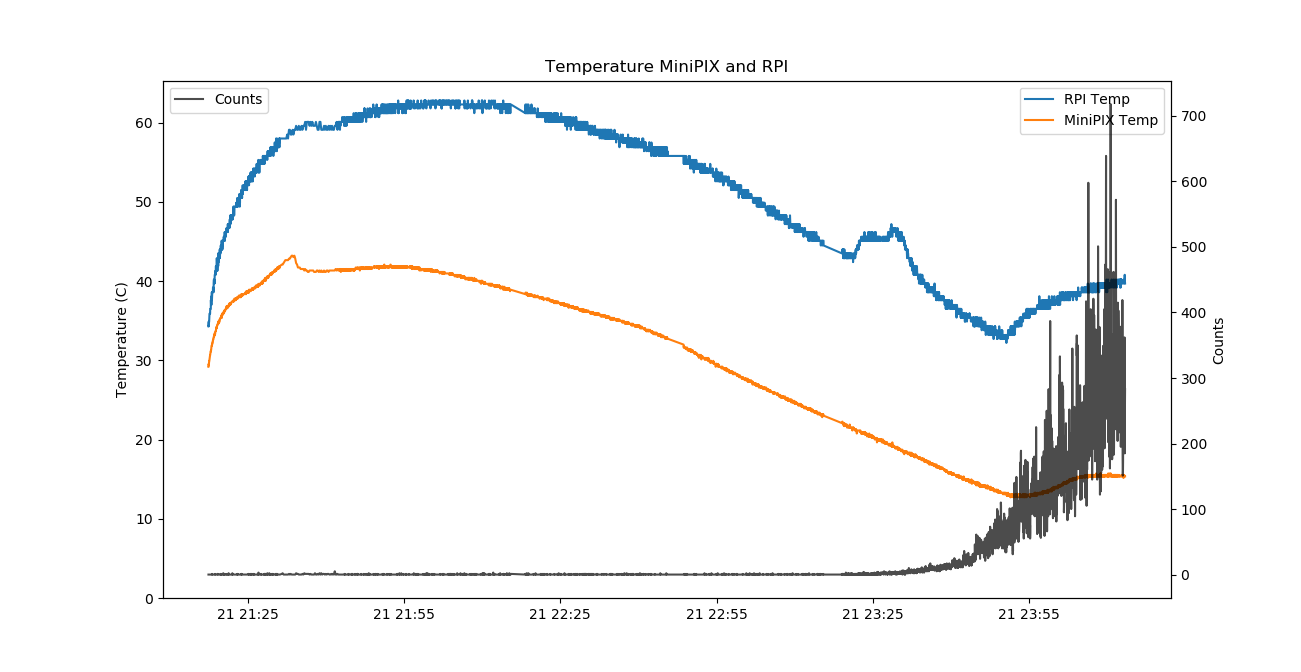
\includegraphics[width=\textwidth]{figures/tempsandcountsvtime.png}
	\caption{Temperature of flight computer and detector and counts during integration testing in Palestine, TX.}
	\label{fig:integrationtemps}
	\end{center}
\end{figure}
